\documentclass[]{article}
\usepackage{lmodern}
\usepackage{amssymb,amsmath}
\usepackage{ifxetex,ifluatex}
\usepackage{fixltx2e} % provides \textsubscript
\ifnum 0\ifxetex 1\fi\ifluatex 1\fi=0 % if pdftex
  \usepackage[T1]{fontenc}
  \usepackage[utf8]{inputenc}
\else % if luatex or xelatex
  \ifxetex
    \usepackage{mathspec}
  \else
    \usepackage{fontspec}
  \fi
  \defaultfontfeatures{Ligatures=TeX,Scale=MatchLowercase}
\fi
% use upquote if available, for straight quotes in verbatim environments
\IfFileExists{upquote.sty}{\usepackage{upquote}}{}
% use microtype if available
\IfFileExists{microtype.sty}{%
\usepackage{microtype}
\UseMicrotypeSet[protrusion]{basicmath} % disable protrusion for tt fonts
}{}
\usepackage[margin=1in]{geometry}
\usepackage{hyperref}
\hypersetup{unicode=true,
            pdftitle={Distribución espacial de delitos},
            pdfauthor={Marto},
            pdfborder={0 0 0},
            breaklinks=true}
\urlstyle{same}  % don't use monospace font for urls
\usepackage{color}
\usepackage{fancyvrb}
\newcommand{\VerbBar}{|}
\newcommand{\VERB}{\Verb[commandchars=\\\{\}]}
\DefineVerbatimEnvironment{Highlighting}{Verbatim}{commandchars=\\\{\}}
% Add ',fontsize=\small' for more characters per line
\usepackage{framed}
\definecolor{shadecolor}{RGB}{248,248,248}
\newenvironment{Shaded}{\begin{snugshade}}{\end{snugshade}}
\newcommand{\AlertTok}[1]{\textcolor[rgb]{0.94,0.16,0.16}{#1}}
\newcommand{\AnnotationTok}[1]{\textcolor[rgb]{0.56,0.35,0.01}{\textbf{\textit{#1}}}}
\newcommand{\AttributeTok}[1]{\textcolor[rgb]{0.77,0.63,0.00}{#1}}
\newcommand{\BaseNTok}[1]{\textcolor[rgb]{0.00,0.00,0.81}{#1}}
\newcommand{\BuiltInTok}[1]{#1}
\newcommand{\CharTok}[1]{\textcolor[rgb]{0.31,0.60,0.02}{#1}}
\newcommand{\CommentTok}[1]{\textcolor[rgb]{0.56,0.35,0.01}{\textit{#1}}}
\newcommand{\CommentVarTok}[1]{\textcolor[rgb]{0.56,0.35,0.01}{\textbf{\textit{#1}}}}
\newcommand{\ConstantTok}[1]{\textcolor[rgb]{0.00,0.00,0.00}{#1}}
\newcommand{\ControlFlowTok}[1]{\textcolor[rgb]{0.13,0.29,0.53}{\textbf{#1}}}
\newcommand{\DataTypeTok}[1]{\textcolor[rgb]{0.13,0.29,0.53}{#1}}
\newcommand{\DecValTok}[1]{\textcolor[rgb]{0.00,0.00,0.81}{#1}}
\newcommand{\DocumentationTok}[1]{\textcolor[rgb]{0.56,0.35,0.01}{\textbf{\textit{#1}}}}
\newcommand{\ErrorTok}[1]{\textcolor[rgb]{0.64,0.00,0.00}{\textbf{#1}}}
\newcommand{\ExtensionTok}[1]{#1}
\newcommand{\FloatTok}[1]{\textcolor[rgb]{0.00,0.00,0.81}{#1}}
\newcommand{\FunctionTok}[1]{\textcolor[rgb]{0.00,0.00,0.00}{#1}}
\newcommand{\ImportTok}[1]{#1}
\newcommand{\InformationTok}[1]{\textcolor[rgb]{0.56,0.35,0.01}{\textbf{\textit{#1}}}}
\newcommand{\KeywordTok}[1]{\textcolor[rgb]{0.13,0.29,0.53}{\textbf{#1}}}
\newcommand{\NormalTok}[1]{#1}
\newcommand{\OperatorTok}[1]{\textcolor[rgb]{0.81,0.36,0.00}{\textbf{#1}}}
\newcommand{\OtherTok}[1]{\textcolor[rgb]{0.56,0.35,0.01}{#1}}
\newcommand{\PreprocessorTok}[1]{\textcolor[rgb]{0.56,0.35,0.01}{\textit{#1}}}
\newcommand{\RegionMarkerTok}[1]{#1}
\newcommand{\SpecialCharTok}[1]{\textcolor[rgb]{0.00,0.00,0.00}{#1}}
\newcommand{\SpecialStringTok}[1]{\textcolor[rgb]{0.31,0.60,0.02}{#1}}
\newcommand{\StringTok}[1]{\textcolor[rgb]{0.31,0.60,0.02}{#1}}
\newcommand{\VariableTok}[1]{\textcolor[rgb]{0.00,0.00,0.00}{#1}}
\newcommand{\VerbatimStringTok}[1]{\textcolor[rgb]{0.31,0.60,0.02}{#1}}
\newcommand{\WarningTok}[1]{\textcolor[rgb]{0.56,0.35,0.01}{\textbf{\textit{#1}}}}
\usepackage{graphicx,grffile}
\makeatletter
\def\maxwidth{\ifdim\Gin@nat@width>\linewidth\linewidth\else\Gin@nat@width\fi}
\def\maxheight{\ifdim\Gin@nat@height>\textheight\textheight\else\Gin@nat@height\fi}
\makeatother
% Scale images if necessary, so that they will not overflow the page
% margins by default, and it is still possible to overwrite the defaults
% using explicit options in \includegraphics[width, height, ...]{}
\setkeys{Gin}{width=\maxwidth,height=\maxheight,keepaspectratio}
\IfFileExists{parskip.sty}{%
\usepackage{parskip}
}{% else
\setlength{\parindent}{0pt}
\setlength{\parskip}{6pt plus 2pt minus 1pt}
}
\setlength{\emergencystretch}{3em}  % prevent overfull lines
\providecommand{\tightlist}{%
  \setlength{\itemsep}{0pt}\setlength{\parskip}{0pt}}
\setcounter{secnumdepth}{0}
% Redefines (sub)paragraphs to behave more like sections
\ifx\paragraph\undefined\else
\let\oldparagraph\paragraph
\renewcommand{\paragraph}[1]{\oldparagraph{#1}\mbox{}}
\fi
\ifx\subparagraph\undefined\else
\let\oldsubparagraph\subparagraph
\renewcommand{\subparagraph}[1]{\oldsubparagraph{#1}\mbox{}}
\fi

%%% Use protect on footnotes to avoid problems with footnotes in titles
\let\rmarkdownfootnote\footnote%
\def\footnote{\protect\rmarkdownfootnote}

%%% Change title format to be more compact
\usepackage{titling}

% Create subtitle command for use in maketitle
\providecommand{\subtitle}[1]{
  \posttitle{
    \begin{center}\large#1\end{center}
    }
}

\setlength{\droptitle}{-2em}

  \title{Distribución espacial de delitos}
    \pretitle{\vspace{\droptitle}\centering\huge}
  \posttitle{\par}
    \author{Marto}
    \preauthor{\centering\large\emph}
  \postauthor{\par}
      \predate{\centering\large\emph}
  \postdate{\par}
    \date{18/12/2019}


\begin{document}
\maketitle

\hypertarget{delitos-en-la-ciudad-de-buenos-aires}{%
\subsection{Delitos en la Ciudad de Buenos
Aires}\label{delitos-en-la-ciudad-de-buenos-aires}}

En consonancia con la
\href{http://rpubs.com/martinalalu/centralidades-comerciales}{política
de datos abiertos} la Ciudad de Buenos Aires comenzó a publicar
información desagregada sobre distintos tipos de delitos en el
\href{https://mapa.seguridadciudad.gob.ar/}{Mapa del Delito}. Los datos
disponibles abarcan el período 2016-2018.

El objetivo del presente trabajo será analizar la distribución espacial
de los delitos en la Ciudad pudiendo identificar cómo éstos variaron (o
no) a lo largo de los años, si hay diferencia entre los distintos tipos
y barrios. Por último se llevará a cabo un
\href{https://es.wikipedia.org/wiki/I_de_Moran}{Test I de Moran} para
poder medir la autocorrelación espacial de los delitos, es decir si su
distribución es producto del azar o no; y por último se realizará un
modelo de regersión simple para modelar la relación de los delitos con
la distancia a las comisarías (en tanto elementos que teóricamente
deberían disuadir la ocurrencia de delitos).

Los datos fueron scrapeados del
\href{https://mapa.seguridadciudad.gob.ar/}{Mapa del Delito} y
preprocesados para poder confeccionar el análisis.

\begin{Shaded}
\begin{Highlighting}[]
\KeywordTok{library}\NormalTok{(data.table)}
\KeywordTok{library}\NormalTok{(tidyverse)}
\KeywordTok{library}\NormalTok{(sf)}
\KeywordTok{library}\NormalTok{(ggplot2)}
\KeywordTok{library}\NormalTok{(dplyr)}
\KeywordTok{library}\NormalTok{(viridis)}
\KeywordTok{library}\NormalTok{(data.table)}
\KeywordTok{library}\NormalTok{(ggmap)}
\KeywordTok{library}\NormalTok{(janitor)}
\KeywordTok{library}\NormalTok{(ggdark)}
\KeywordTok{library}\NormalTok{(leaflet)}
\KeywordTok{library}\NormalTok{(lubridate)}

\NormalTok{delitos <{-}}\StringTok{ }\KeywordTok{fread}\NormalTok{(}\StringTok{"https://raw.githubusercontent.com/martoalalu/delitos{-}caba/master/data/delitos.csv"}\NormalTok{)}
\NormalTok{delitos <{-}}\StringTok{ }\NormalTok{delitos }\OperatorTok{\%>\%}\StringTok{ }
\StringTok{  }\KeywordTok{mutate}\NormalTok{(}\DataTypeTok{fecha=}\KeywordTok{ymd}\NormalTok{(fecha)) }\OperatorTok{\%>\%}\StringTok{ }
\StringTok{  }\KeywordTok{mutate}\NormalTok{(}\DataTypeTok{anio=}\KeywordTok{year}\NormalTok{(fecha)) }\OperatorTok{\%>\%}\StringTok{ }
\StringTok{  }\KeywordTok{mutate}\NormalTok{(}\DataTypeTok{anio\_mes =} \KeywordTok{floor\_date}\NormalTok{(}\KeywordTok{as\_date}\NormalTok{(fecha), }\StringTok{"month"}\NormalTok{))}

\KeywordTok{nrow}\NormalTok{(delitos)}\OperatorTok{/}\NormalTok{(}\DecValTok{365}\OperatorTok{*}\DecValTok{3}\NormalTok{)}
\end{Highlighting}
\end{Shaded}

\begin{verbatim}
## [1] 320.5297
\end{verbatim}

\begin{Shaded}
\begin{Highlighting}[]
\NormalTok{delitos }\OperatorTok{\%>\%}\StringTok{ }
\StringTok{  }\KeywordTok{count}\NormalTok{(anio) }\OperatorTok{\%>\%}\StringTok{ }
\StringTok{  }\KeywordTok{mutate}\NormalTok{(}\DataTypeTok{pct=}\NormalTok{(n}\OperatorTok{/}\KeywordTok{sum}\NormalTok{(n))}\OperatorTok{*}\DecValTok{100}\NormalTok{)}
\end{Highlighting}
\end{Shaded}

\begin{verbatim}
## # A tibble: 3 x 3
##    anio      n   pct
##   <dbl>  <int> <dbl>
## 1  2016 117675  33.5
## 2  2017 120514  34.3
## 3  2018 112791  32.1
\end{verbatim}

\begin{Shaded}
\begin{Highlighting}[]
\NormalTok{delitos }\OperatorTok{\%>\%}\StringTok{ }
\StringTok{  }\KeywordTok{ggplot}\NormalTok{(}\KeywordTok{aes}\NormalTok{(anio))}\OperatorTok{+}
\StringTok{    }\KeywordTok{geom\_bar}\NormalTok{(}\KeywordTok{aes}\NormalTok{(}\DataTypeTok{fill=}\KeywordTok{as.factor}\NormalTok{(tipo\_delito)))}\OperatorTok{+}
\StringTok{  }\KeywordTok{labs}\NormalTok{(}\DataTypeTok{title=}\StringTok{"Distribución de delitos por año (2016{-}2018)"}\NormalTok{,}
       \DataTypeTok{subtitle=}\StringTok{"Ciudad Autónoma de Buenos Aires"}\NormalTok{,}
       \DataTypeTok{caption=} \StringTok{"Fuente de datos: https://https://mapa.seguridadciudad.gob.ar/"}\NormalTok{,}
       \DataTypeTok{fill=}\StringTok{"Tipo de delito"}\NormalTok{)}
\end{Highlighting}
\end{Shaded}

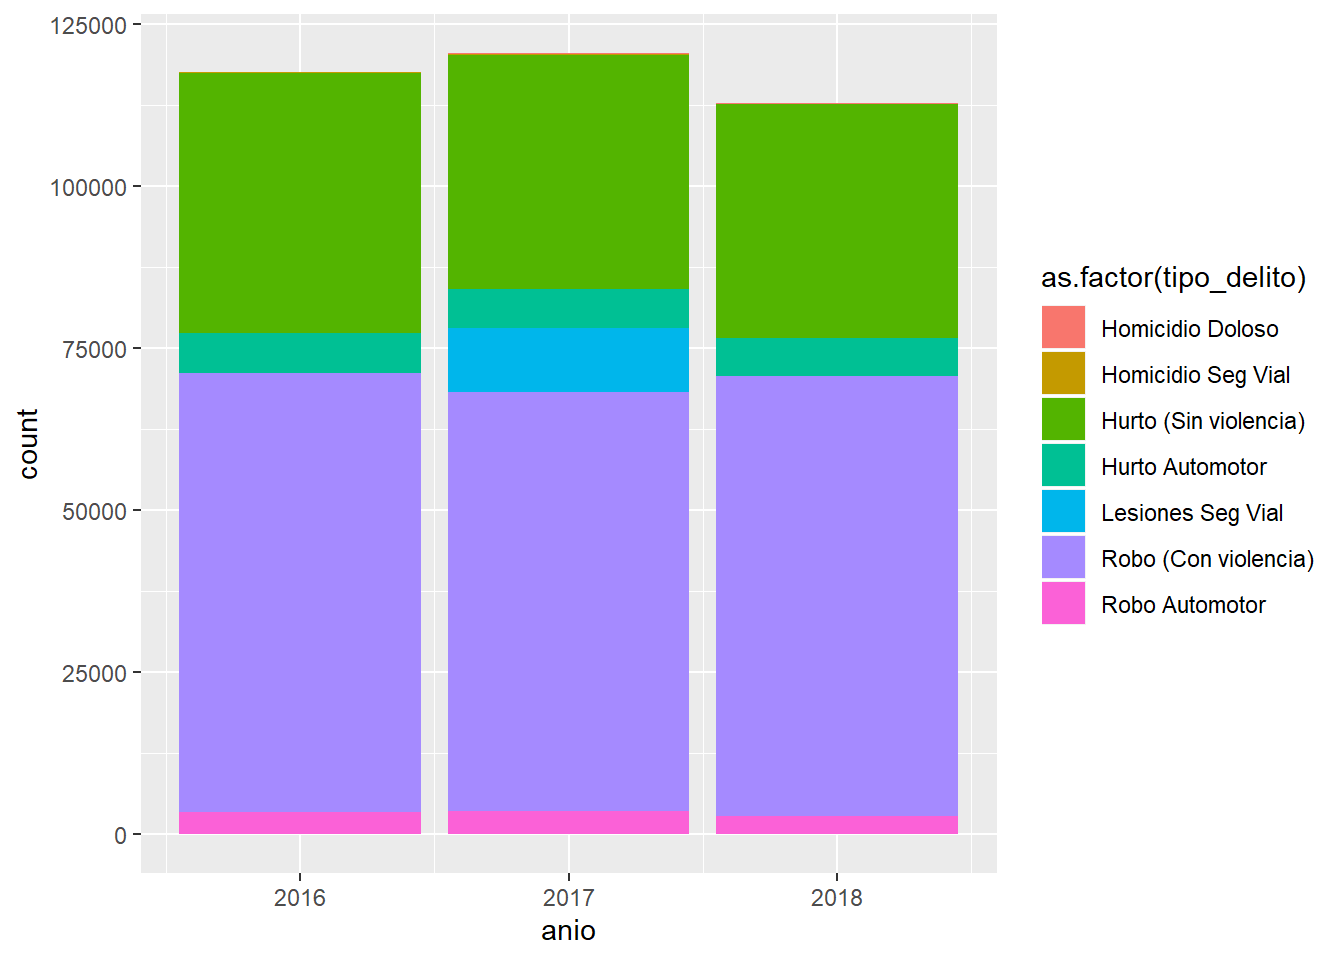
\includegraphics{delitos-caba_files/figure-latex/unnamed-chunk-1-1.pdf}

En los 3 años se cometieron \textbf{350980 delitos}, un promedio de
\textbf{320 por día}, mientras que la distribución en este período es
bastante pareja, con un 33.5\% en 2016, 34.3\% en 2017 y 32.1\% en 2018.
Mientras que en cuanto a los tipos de delito tampoco hay grandes
variaciones, con amplia predominancia de \textbf{Robo con violencia} y
\textbf{Hurto sin violencia}, la irrupción de \textbf{Lesiones en
seguridad vial} en 2017 se explica únicamente porque es el único período
con datos de ese tipo de delito.

\begin{Shaded}
\begin{Highlighting}[]
\NormalTok{delitos }\OperatorTok{\%>\%}\StringTok{ }
\StringTok{  }\KeywordTok{count}\NormalTok{(anio\_mes,tipo\_delito) }\OperatorTok{\%>\%}\StringTok{ }
\StringTok{  }\KeywordTok{ggplot}\NormalTok{() }\OperatorTok{+}
\StringTok{  }\KeywordTok{geom\_line}\NormalTok{(}\KeywordTok{aes}\NormalTok{(}\DataTypeTok{x=}\NormalTok{anio\_mes, }\DataTypeTok{y=}\NormalTok{n, }\DataTypeTok{color=}\NormalTok{tipo\_delito))}\OperatorTok{+}
\StringTok{  }\KeywordTok{xlab}\NormalTok{(}\StringTok{""}\NormalTok{)}\OperatorTok{+}
\StringTok{  }\KeywordTok{labs}\NormalTok{(}\DataTypeTok{title=}\StringTok{"Distribución de delitos por mes (2016{-}2018)"}\NormalTok{,}
       \DataTypeTok{subtitle=}\StringTok{"Ciudad Autónoma de Buenos Aires"}\NormalTok{,}
       \DataTypeTok{caption=} \StringTok{"Fuente de datos: https://https://mapa.seguridadciudad.gob.ar/"}\NormalTok{,}
       \DataTypeTok{fill=}\StringTok{"Tipo de delito"}\NormalTok{)}
\end{Highlighting}
\end{Shaded}

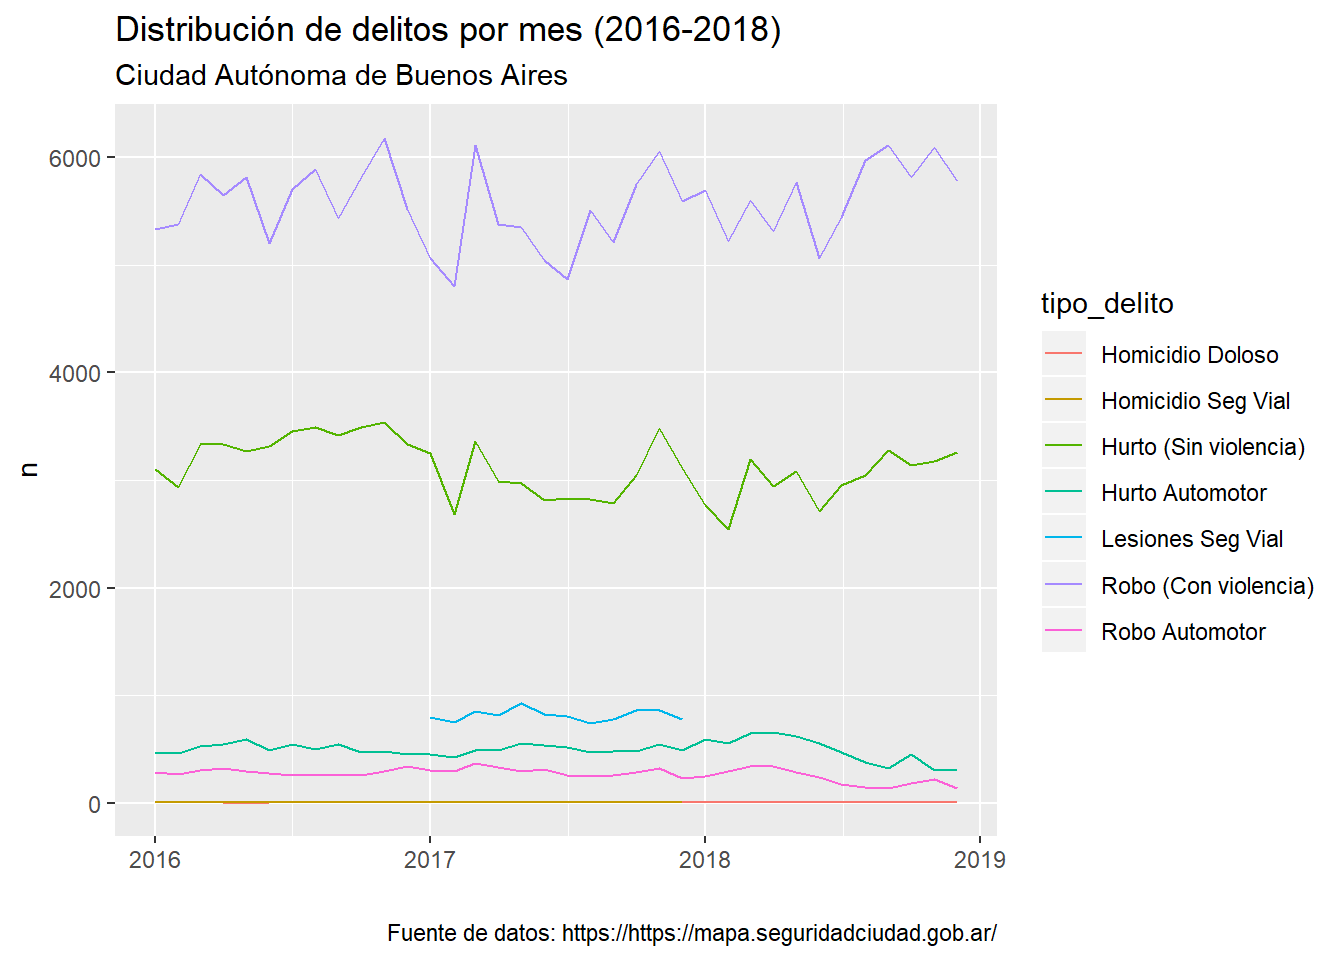
\includegraphics{delitos-caba_files/figure-latex/unnamed-chunk-2-1.pdf}

En términos generales no se observan grandes variaciones a lo largo del
período, la cantidad de delitos se mantiene a pesar de las fluctiaciones
durante el año. A fines prácticos en el presente trabajo nos
concentraremos en los dos principales delitos de este período,
\textbf{Robo (Con violencia) con 200374 hechos} y \textbf{Hurto (Sin
violencia) con 112301 hechos},los cuales \textbf{concentran el 89\% del
total de los delitos} en el período analizado.

\hypertarget{distribucion-espacial}{%
\section{Distribución espacial}\label{distribucion-espacial}}

Veamos cómo fue la distribución espacial de estos delitos a lo largo de
los 3 años.

\begin{Shaded}
\begin{Highlighting}[]
\CommentTok{\#Creamos df con delitos de robo y hurto que tengan coordenadas}
\NormalTok{delitos\_geo <{-}}\StringTok{ }\NormalTok{delitos }\OperatorTok{\%>\%}\StringTok{ }
\StringTok{  }\KeywordTok{filter}\NormalTok{(}\OperatorTok{!}\KeywordTok{is.na}\NormalTok{(longitud), }\OperatorTok{!}\KeywordTok{is.na}\NormalTok{(latitud)) }\OperatorTok{\%>\%}
\StringTok{  }\KeywordTok{filter}\NormalTok{(longitud }\OperatorTok{!=}\StringTok{ }\DecValTok{0}\NormalTok{) }\OperatorTok{\%>\%}
\StringTok{  }\KeywordTok{filter}\NormalTok{(tipo\_delito}\OperatorTok{==}\StringTok{"Robo (Con Violencia)"} \OperatorTok{|}\StringTok{ }\NormalTok{tipo\_delito}\OperatorTok{==}\StringTok{"Hurto (Sin violencia)"}\NormalTok{) }\OperatorTok{\%>\%}\StringTok{ }
\StringTok{  }\KeywordTok{st\_as\_sf}\NormalTok{(}\DataTypeTok{coords =} \KeywordTok{c}\NormalTok{(}\StringTok{"longitud"}\NormalTok{, }\StringTok{"latitud"}\NormalTok{), }\DataTypeTok{crs =} \DecValTok{4326}\NormalTok{)}

\CommentTok{\#Nos quedamos solo con los delitos ocurridos en la Ciudad de Buenos Aires}
\NormalTok{radios <{-}}\StringTok{ }\KeywordTok{read\_sf}\NormalTok{(}\StringTok{"http://cdn.buenosaires.gob.ar/datosabiertos/datasets/informacion{-}censal{-}por{-}radio/caba\_radios\_censales.geojson"}\NormalTok{)}

\NormalTok{delitos\_caba <{-}}\StringTok{ }\NormalTok{delitos\_geo[}\KeywordTok{st\_within}\NormalTok{(delitos\_geo, radios) }\OperatorTok{\%>\%}\StringTok{ }\NormalTok{lengths }\OperatorTok{>}\StringTok{ }\DecValTok{0}\NormalTok{,]}
\end{Highlighting}
\end{Shaded}

Luego del filtro nos quedamos con un total de 110822 delitos.

When you click the \textbf{Knit} button a document will be generated
that includes both content as well as the output of any embedded R code
chunks within the document. You can embed an R code chunk like this:

\begin{Shaded}
\begin{Highlighting}[]
\KeywordTok{summary}\NormalTok{(cars)}
\end{Highlighting}
\end{Shaded}

\begin{verbatim}
##      speed           dist       
##  Min.   : 4.0   Min.   :  2.00  
##  1st Qu.:12.0   1st Qu.: 26.00  
##  Median :15.0   Median : 36.00  
##  Mean   :15.4   Mean   : 42.98  
##  3rd Qu.:19.0   3rd Qu.: 56.00  
##  Max.   :25.0   Max.   :120.00
\end{verbatim}

\hypertarget{including-plots}{%
\subsection{Including Plots}\label{including-plots}}

You can also embed plots, for example:

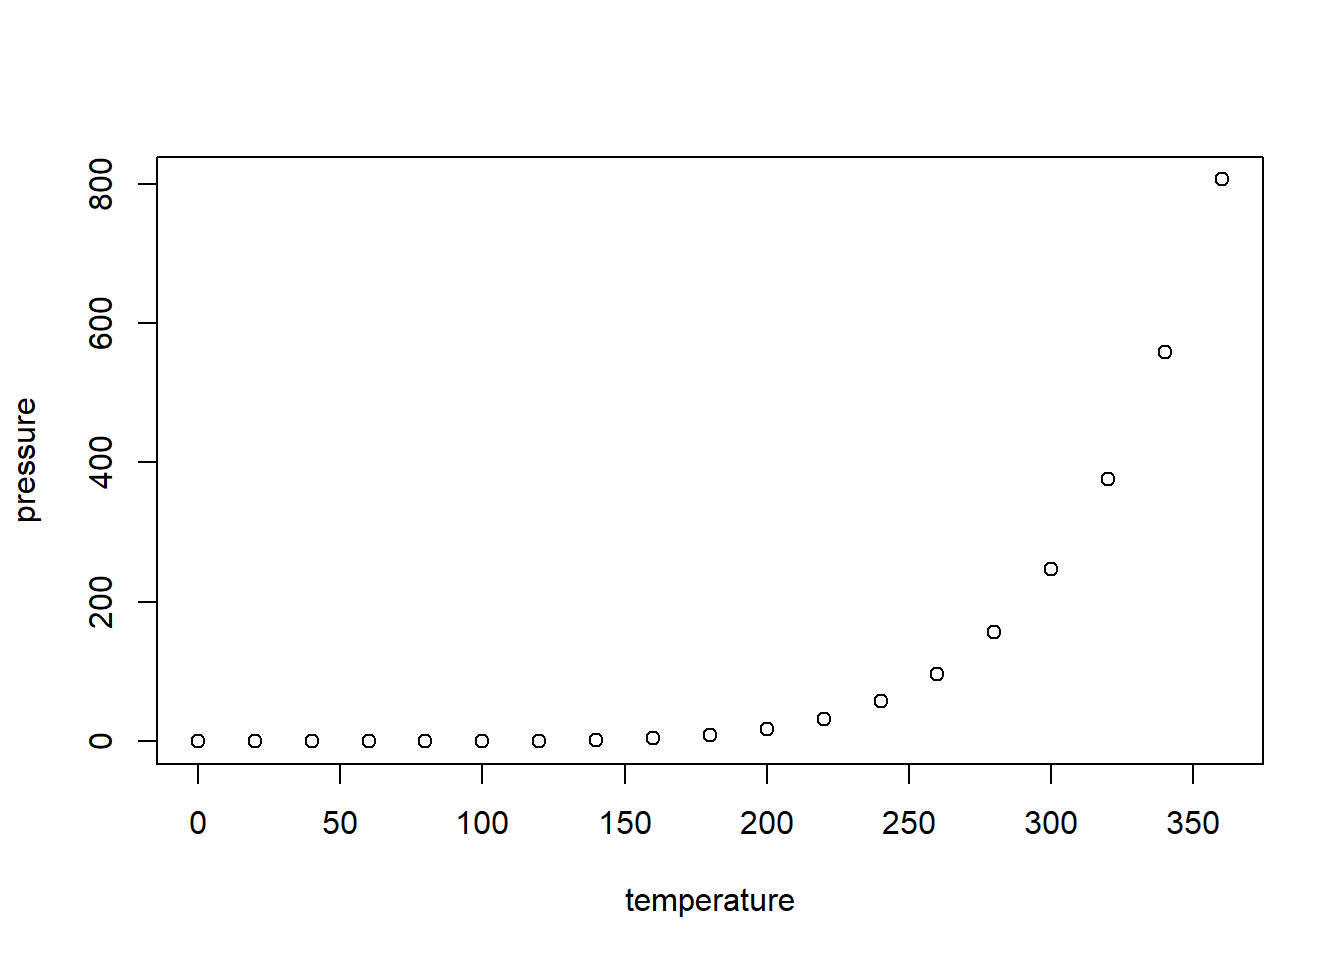
\includegraphics{delitos-caba_files/figure-latex/pressure-1.pdf}

Note that the \texttt{echo\ =\ FALSE} parameter was added to the code
chunk to prevent printing of the R code that generated the plot.


\end{document}
